\newcommand{\app}{\raise.17ex\hbox{$\scriptstyle\sim$}}
\newcommand{\ncdot}{{\mkern 0mu\cdot\mkern 0mu}}
\def\x{\times}

\newcolumntype{x}[1]{>{\centering\arraybackslash}p{#1pt}}
\newcommand{\dt}[1]{\fontsize{8pt}{.1em}\selectfont \emph{#1}}
% \newlength\savewidth
\renewcommand\shline{\noalign{\global\savewidth\arrayrulewidth
  \global\arrayrulewidth 1pt}\hline\noalign{\global\arrayrulewidth\savewidth}}
\newcommand{\tablestyle}[2]{\setlength{\tabcolsep}{#1}\renewcommand{\arraystretch}{#2}\centering\footnotesize}
\makeatletter\renewcommand\paragraph{\@startsection{paragraph}{4}{\z@}
  {.5em \@plus1ex \@minus.2ex}{-.5em}{\normalfont\normalsize\bfseries}}\makeatother

\xjtuappendixchapter{外文文献翻译}

\begin{center}
    \sihao\textbf{Spring 框架使用文档}
\end{center}

\xjtuappendixsection{控制反转容器}

这一节介绍了Spring实现控制反转的准则。控制反转为依赖注入而知名。依赖注入指各个对象仅仅通过各自构造函数、工厂方法的参数的方式声明自己的依赖(依赖是它们正常工作所需要其他对象)。你也可以在对象构造器构造完毕后或由工厂方法返回之后,使用 setter 方法来声明依赖。这个过程从根本上将对象构建依赖的顺序倒转了过来,由外部管理对象依赖而不是由对象资深实例化依赖。

包 org.springframework.beans 以及包org.springframework.context 是 Spring控制反转容器的基础。同时, BeanFactory 接口提供了一种高级的管理机制可以用来管理任何类型的对象。ApplicationContext 是 BeanFactory 的子接口,它增加了以下特性:

\begin{itemize}
  \item 更加易于与 Spring 面向切面编程特性整合
  \item 消息资源处理机制
  \item 事件发布
  \item 应用层面特别上下文
\end{itemize}

简而言之,BeanFactory 提供配置框架与基础功能,而 ApplicationContext 添加了一些更加企业化的功能。ApplicationContext 是 BeanFactory 的一个超集。

在 Spring 中,对象是你的应用主体,且它们都被 Spring 控制反转容器所管理,我们将它们称之为 bean。bean 是一种由控制反转容器进行初始化、装配的对象。通常你的应用中大部分对象都应该是 bean。通常 bean 和它们的依赖都是配置在控制反转容器中。

\xjtuappendixsubsection{配置数据}
org.springframework.context.ApplicationContext 接口代表了一个 Spring 控制反转容器并且负责初始化、配置以及装配 bean。容器通过读取它的配置文件来进行判断对那些对象进行初始化、装配或配置。配置元数据可以由 XML、Java 注解或Java 代码来表示。这样你就可以将你的应用中的对象以及它们的依赖表示出来。

Spring 提供了 ApplicationContext 接口的一些实现。在一个独立的应用中,我们通常创建 ClassPathXmlApplicationContext 或 FileSystemApplicationContext 的实例作为容器。在 XML 作为传统配置文件的同时,你也可以使用 Java 注解或代码来定义配置。

在大多数应用场景中,并不需要用户去显式地实例化一个或多个 Spring 控制反转容器,如一个简单的 Web 应用中,容器是通过 web.xml 定义的。如果你使用Spring工具套件,你可以轻松地哦通过点击鼠标或快捷键来定义这些配置。

图 \ref{fig:spring-di} 从较高的层次上展示了Spring是如何工作的。你的应用中的类与配置文件就是这样结合在一起的。在ApplicationContext 被创建及初始化后,你就有了一个配置完毕的可以直接使用的应用。

\begin{figure}[!ht]
  \centering
  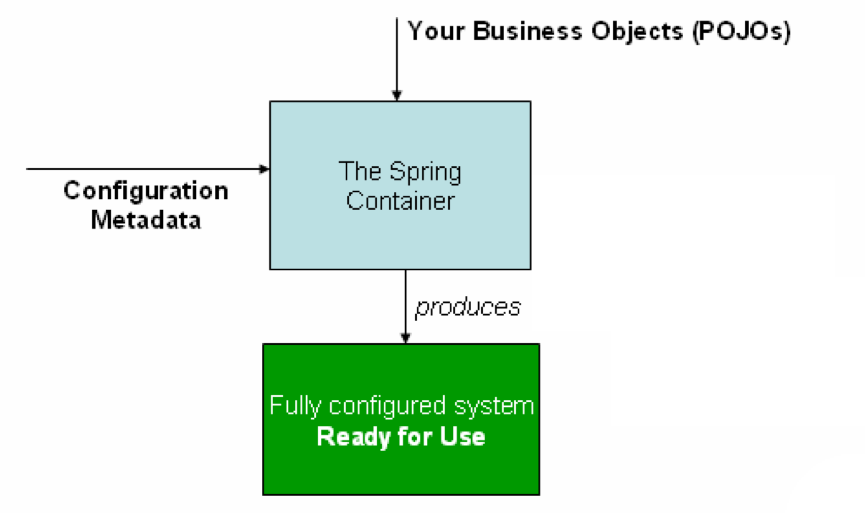
\includegraphics[width=0.7\textwidth]{翻译.png}
  \caption{Spring 依赖注入工作流程}
  \label{fig:spring-di}
\end{figure}

正如流程图 \ref{fig:spring-di} 所示,Spring控制反转容器需要一定格式的配置元数据。这些配置元数据表明了作为一个应用开发者,你是如何通过何种方式告知 Spring 容器去在你的应用中,实例化、装配各种对象。

配置元数据传统上通过一个简单的、符合直觉的XML文件提供,在本章中我们也用 XML 来白表达关键概念以及Spring控制反转容器的特性。

Spring配置文件通常至少包含一个 bean 的定义,通常情况下包含多个 bean 定义。在基于XML的配置元数据中 bean是通过包含在<beans/>中的<bean/>元素来定义的。使用Java配置时通常使用@Bean注解,配置文件就是经@Configuration注解的Java类。

这些bean的配置与组成应用的实际对象紧密相关。很多时候,你会定义服务层对象、数据存取对象、表现对象如:Struts框架中的Action实例、基础对象如:Hinernate框架中的SessionFactories对象,JMS框架中的Queues对象,等等。一般来说,人们并不会在容器中定义应用的领域对象,创建与装载领域对象是数据存取层与商务逻辑的职责。然而,你可以将Spring与AspectJ整合起来去配置在控制反转容器之外创建的对象。

图 \ref{fig:spring-code-1} 展示了基于XML的配置元数据的基础结构:

\begin{figure}[!ht]
  \centering
  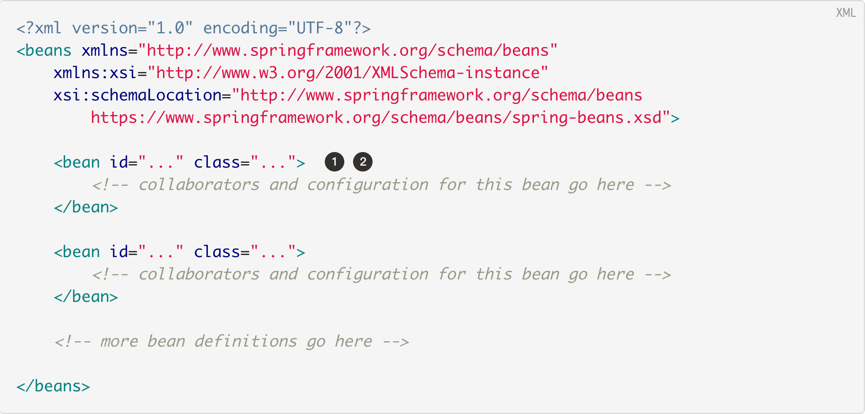
\includegraphics[width=1\textwidth]{code-1.png}
  \caption{XML 配置数据}
  \label{fig:spring-code-1}
\end{figure}

其中id属性是一个用于识别每个独立bean定义的字符串。class属性定义了bean的类型以及相对应的具体类。id属性的值可以用来协助各个对象之间的合作。

\xjtuappendixsubsection{实例化一个容器}

如图 \ref{fig:spring-code-2} 所示,我们可以向ApplicationContext的构造器中传入一个或多个路径,这些路径是一些资源字符串,可以让容器从各种外部资源中获取配置元数据,比如从文件系统中获取、Java的CLASSPATH获取等。

\begin{figure}[!ht]
  \centering
  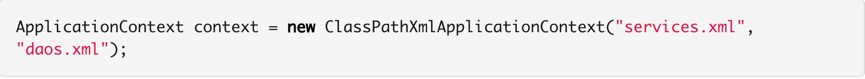
\includegraphics[width=1\textwidth]{code-2.png}
  \caption{加载配置数据}
  \label{fig:spring-code-2}
\end{figure}

在你学习了Spring控制反转容器之后,你可能希望了解更多关于Spring资源抽象的概念。资源抽象提供了一种方便的机制来从指定的URI中读取输入流。尤其,资源路径被用来构建应用上下文。

图 \ref{fig:spring-code-3} 展示了服务层对象的配置文件:

\begin{figure}[!ht]
  \centering
  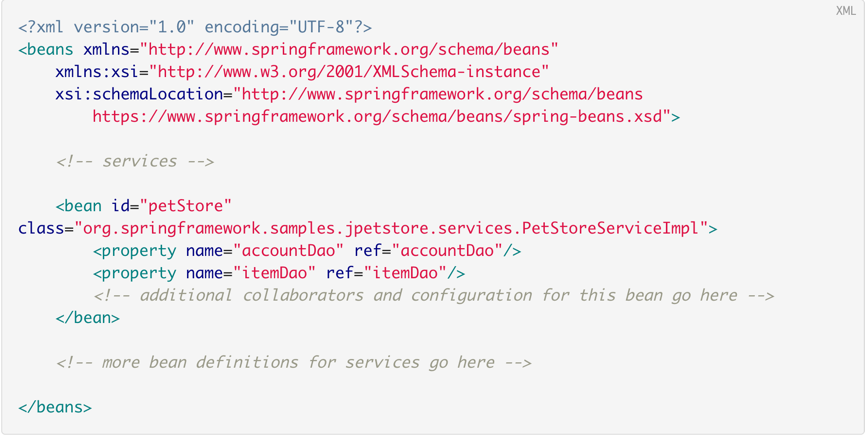
\includegraphics[width=1\textwidth]{code-3.png}
  \caption{服务层对象配置}
  \label{fig:spring-code-3}
\end{figure}

在上述的例子中,服务层包含PetStoreServiceImpl类以及两个数据访问对象,分别是JpaAccountDao和JpaItemDao。name元素指向此bean的所有属性值得名称。同时ref元素代指bean定义中属性的具体值。id与ref之间的联系表示了合作对象之间的依赖

有时有多个定义bean的XML文件会很有用。通常情况下XML配置文件代表了一个应用中的逻辑层或一个模块。

你可以使用通过应用上下文来从这些XML片段中读取bean的定义信息。上下文的构造器传入多个资源位置,正如前一节所示。或者,使用一个或多个<import/>标签来载入多个文件中的bean定义。

如图 \ref{fig:spring-code-4} 所示,外部的bean定义来自services.xml,messageSource.xml以及themeSource.xml。所有的路径地址都是相对于这个执行导入操作的文件的。所以,services.xml必须和导入文件在同一目录或位于CLASSPATH下,同时messageSource.xml和themeSource.xml必须位于导入文件同级目录下的resources目录下。正如你所看见的,路径中最前面的斜杠被忽略了。然而,当路径为绝对路径时不要在路径最前面加斜杠。上述文件的内容一杯导入进来,根据Spring的模式,在最顶级的<beans/>标签内所有的bean定义都是有效的。

\begin{figure}[!ht]
  \centering
  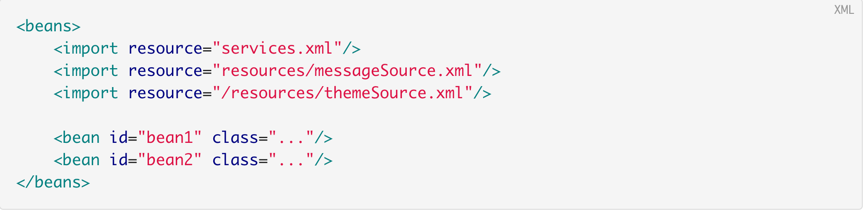
\includegraphics[width=1\textwidth]{code-4.png}
  \caption{配置中引入其他配置文件}
  \label{fig:spring-code-4}
\end{figure}

你可以使用相对路径中的 ../ 来指向父目录中的文件,但我们不推荐这么做。这样做的话应用就对应用外的事物产生了依赖。尤其,这种做法不应该用于在使用类路径URL的时候,如:classpath:../services.xml,因为运行时解析进程会选择一个最近的类根路径再到其父目录中查找。当类路径配置改变时可能会导致一个不同的、有误的目录。

你可以一直使用全路径名代替相对路径名。比如:file:C:/config/services.xml或classpath:/config/services.xml。然而,你要注意到里的应用配置已经和某个绝对路径联系到一起了。通常情况下,我们并不会直接使用一个绝对路径,而是通过 \$\{…\} 占位符来使用,这样可以在运行时由解析系统解析。

XML文件中各命名空间引入了一些直接的特性。在普通的bean定义之上的各种高级配置特性都可以通过Spring所提供的命名空间所使用,如:context命名空间以及util命名空间。

这是一个用于展示扩展的配置元数据的更深远的例子,就像Grails框架一样,bean的定义同样可以使用Spring Groovy Bean定义语句来表示。通常,这些配置卸载一个 .groovy文件中,格式见图 \ref{fig:spring-code-5}:

\begin{figure}[!ht]
  \centering
  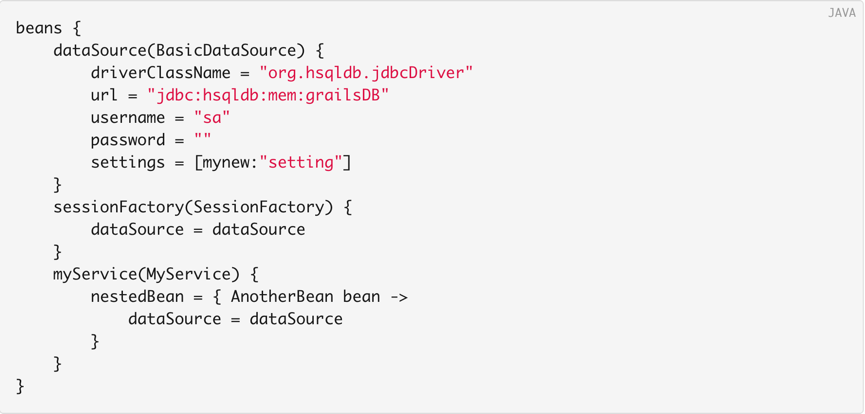
\includegraphics[width=1\textwidth]{code-5.png}
  \caption{通过 Groovy 配置 Beans}
  \label{fig:spring-code-5}
\end{figure}

这种配置方式的风格很大程度上与XML是等价的,甚至它支持Spring XML的命名空间。它也允许你在其中通过importBeans语句导入XML bean定义文件。

\xjtuappendixsubsection{使用容器}
ApplicationContext是一个接口,它可以用于在一个高级工厂类中维持一个各种类以及它们的依赖的注册信息。通过使用T getBean(String name, Class<T> requiredType) 方法,你就可以获取到你需要的bean的实例。

ApplicationContext可以让你阅读bean的定义以及获取一个bean,例子如图 \ref{fig:spring-code-6} 所示:

\begin{figure}[!ht]
  \centering
  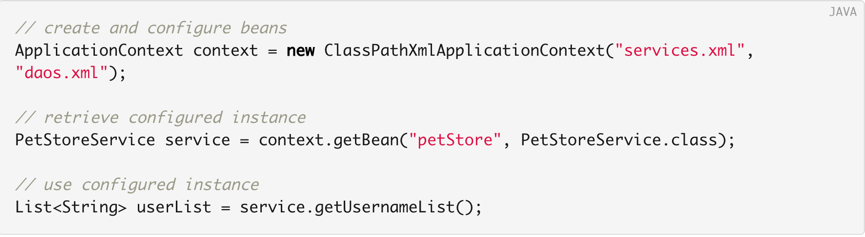
\includegraphics[width=1\textwidth]{code-6.png}
  \caption{Spring 读取配置文件}
  \label{fig:spring-code-6}
\end{figure}

\xjtuappendixsection{Bean 总览}

每一个 Spring 控制反转容器都管理一个或多个 bean。这些 bean 是通过你提供给容器的元数据而创建的(例如:通过 XML 中的 <bean/> 的形式)。

在容器中,这些 bean 的定义表现为许多 BeanDefinition 对象。其中每个对象包含以下元数据:

\begin{itemize}
  \item 一个包含包名的类全限定名:通常情况下,实际的 bean 的时限内已被定义。
  \item Bean 的行为配置元素,即在容器中 bean 的每个状态有何表现(作用域、生命周期回调、等等)。
  \item 指向 bean 工作所必须的其他 bean 的引用。这些引用也叫合作者或依赖。
  \item 需要在新生成的对象中设置的其他配置选项。比如:在连接池管理 bean 中的连接池的大小、 bean 中使用的连接的数量。
\end{itemize}

这些元数据可以被转换为一系列属性,从而组成每个 bean 的定义。表 \ref{tab:bean} 列出了这些属性:

\begin{table}[!ht]
  \centering
  \caption{bean 属性表}
\label{tab:bean}
  \begin{tabularx}{\textwidth}{p{0.5\textwidth}<{\centering}p{0.5\textwidth}<{\centering}}
  \toprule
  Property & Explained in \\ \midrule
  Class & Instantiating Beans \\
  Name & Naming Beans \\ 
  Scope & Bean Scopes \\ 
  Constructor arguments & Dependency injection \\ 
  Properties & Dependency injection \\ 
  Autowiring mode & Autowiring Collaborators \\ 
  Lazy initialization mode & Lazy-initialized Beans \\ 
  initialization method & Initialization Callbacks \\
  Destruction method & Destruction Callbacks \\ \bottomrule
  \end{tabularx}
\end{table}




\xjtuappendixchapter{外文文献原文}

\begin{center}
    \sihao\textbf{Spring Framework Documentation}
\end{center}

\xjtuappendixsection{The IoC Container}

This chapter covers the Spring Framework implementation of the Inversion of Control (IoC) principle. IoC is also known as dependency injection (DI). It is a process whereby objects define their dependencies (that is, the other objects they work with) only through constructor arguments, arguments to a factory method, or properties that are set on the object instance after it is constructed or returned from a factory method. The container then injects those dependencies when it creates the bean. This process is fundamentally the inverse (hence the name, Inversion of Control) of the bean itself controlling the instantiation or location of its dependencies by using direct construction of classes or a mechanism such as the Service Locator pattern.

The org.springframework.beans and org.springframework.context packages are the basis for Spring Framework’s IoC container. The BeanFactory interface provides an advanced configuration mechanism capable of managing any type of object. ApplicationContext is a sub-interface of BeanFactory. It adds:

\begin{itemize}
  \item Easier integration with Spring's AOP features
  \item Message resource handling (for use in internationalization)
  \item Event publication
  \item Application-layer specific contexts such as the WebApplicationContext for use in web applications.
\end{itemize}

the BeanFactory provides the configuration framework and basic functionality, and the \hyphenation{App-lication-Con-text} adds more enterprise-specific functionality. \hyphenation{App-lication-Con-text} a complete superset of the \hyphenation{Bean-Factory} and is used exclusively in this chapter in descriptions of Spring’s IoC container. For more information on using the \hyphenation{Bean-Factory} instead of \hyphenation{App-lication-Con-text}, see The \hyphenation{Bean-Factory}.

In Spring, the objects that form the backbone of your application and that are managed by the Spring IoC container are called beans. A bean is an object that is instantiated, assembled, and otherwise managed by a Spring IoC container. Otherwise, a bean is simply one of many objects in your application. Beans, and the dependencies among them, are reflected in the configuration metadata used by a container.

\xjtuappendixsubsection{Configuration Metadata}

The org.springframework.context.ApplicationContext interface represents the Spring IoC container and is responsible for instantiating, configuring, and assembling the beans. The container gets its instructions on what objects to instantiate, configure, and assemble by reading configuration metadata. The configuration metadata is represented in XML, Java annotations, or Java code. It lets you express the objects that compose your application and the rich interdependencies between those objects.

Several implementations of the ApplicationContext interface are supplied with Spring. In stand-alone applications, it is common to create an instance. While XML has been the traditional format for defining configuration metadata, you can instruct the container to use Java annotations or code as the metadata format by providing a small amount of XML configuration to declaratively enable support for these additional metadata formats.

In most application scenarios, explicit user code is not required to instantiate one or more instances of a Spring IoC container. For example, in a web application scenario, a simple eight (or so) lines of boilerplate web descriptor XML in the web.xml file of the application typically suffices (see Convenient ApplicationContext Instantiation for Web Applications). If you use the Spring Tool Suite (an Eclipse-powered development environment), you can easily create this boilerplate configuration with a few mouse clicks or keystrokes.

Diagram \ref{fig:spring-di-en} shows a high-level view of how Spring works. Your application classes are combined with configuration metadata so that, after the ApplicationContext is created and initialized, you have a fully configured and executable system or application.

\begin{figure}[!ht]
  \centering
  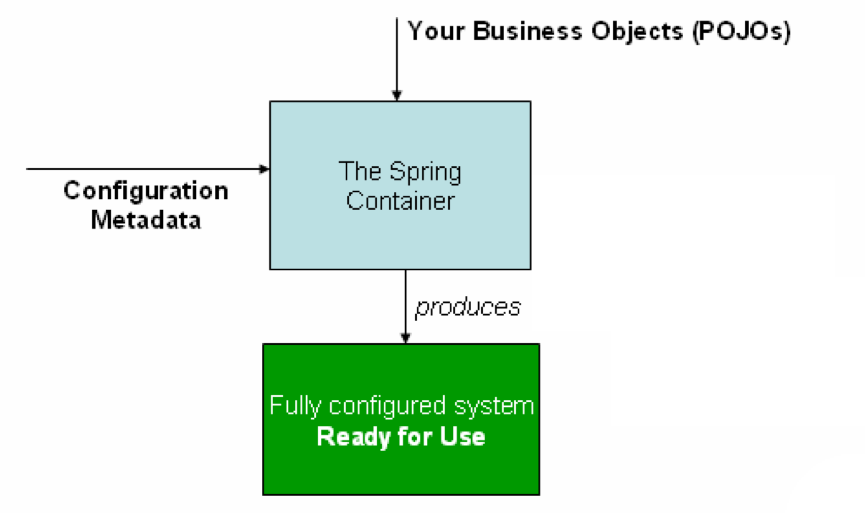
\includegraphics[width=0.7\textwidth]{翻译.png}
  \caption{The Spring IoC container}
  \label{fig:spring-di-en}
\end{figure}

As the preceding diagram shows, the Spring IoC container consumes a form of configuration metadata. This configuration metadata represents how you, as an application developer, tell the Spring container to instantiate, configure, and assemble the objects in your application.

Configuration metadata is traditionally supplied in a simple and intuitive XML format, which is what most of this chapter uses to convey key concepts and features of the Spring IoC container.

XML-based metadata is not the only allowed form of configuration metadata. The Spring IoC container itself is totally decoupled from the format in which this configuration metadata is actually written. These days, many developers choose Java-based configuration for their Spring applications.

Spring configuration consists of at least one and typically more than one bean definition that the container must manage. XML-based configuration metadata configures these beans as <bean/> elements inside a top-level <beans/> element. Java configuration typically uses @Bean-annotated methods within a @Configuration class.

These bean definitions correspond to the actual objects that make up your application. Typically, you define service layer objects, data access objects (DAOs), presentation objects such as Struts Action instances, infrastructure objects such as Hibernate SessionFactories, and so forth. Typically, one does not configure fine-grained domain objects in the container, because it is usually the responsibility of DAOs and business logic to create and load domain objects. However, you can use Spring’s integration with AspectJ to configure objects that have been created outside the control of an IoC container. See Using AspectJ to dependency-inject domain objects with Spring.

Picture \ref{fig:spring-code-1-en} shows the basic structure of XML-based configuration metadata:

\begin{figure}[!ht]
  \centering
  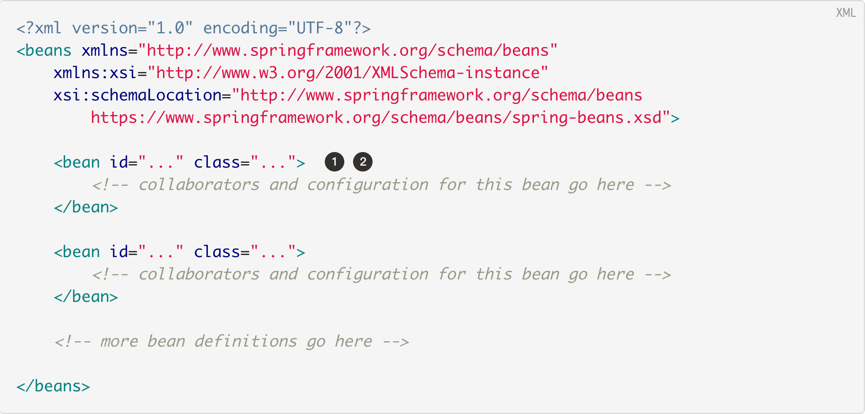
\includegraphics[width=1\textwidth]{code-1.png}
  \caption{Basic structure of XML-based configuration metadata}
  \label{fig:spring-code-1-en}
\end{figure}


The id attribute is a string that identifies the individual bean definition.

The class attribute defines the type of the bean and uses the fully qualified classname.The value of the id attribute refers to collaborating objects. The XML for referring to collaborating objects is not shown in this example. See Dependencies for more information.

\xjtuappendixsubsection{Instantiating a Container}
The location path or paths supplied to an ApplicationContext constructor are resource strings that let the container load configuration metadata from a variety of external resources, such as the local file system, the Java CLASSPATH, and so on, as the picture \ref{fig:spring-code-2-en}.

\begin{figure}[!ht]
  \centering
  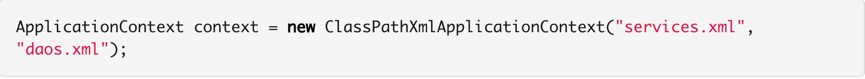
\includegraphics[width=1\textwidth]{code-2.png}
  \caption{加Loading metadata}
  \label{fig:spring-code-2-en}
\end{figure}


After you learn about Spring’s IoC container, you may want to know more about Spring’s Resourceabstraction (as described in Resources), which provides a convenient mechanism for reading an InputStream from locations defined in a URI syntax. In particular, Resource paths are used to construct applications contexts, as described in Application Contexts and Resource Paths.
Picture \ref{fig:spring-code-3-en} shows the service layer objects (services.xml) configuration file:

\begin{figure}[!ht]
  \centering
  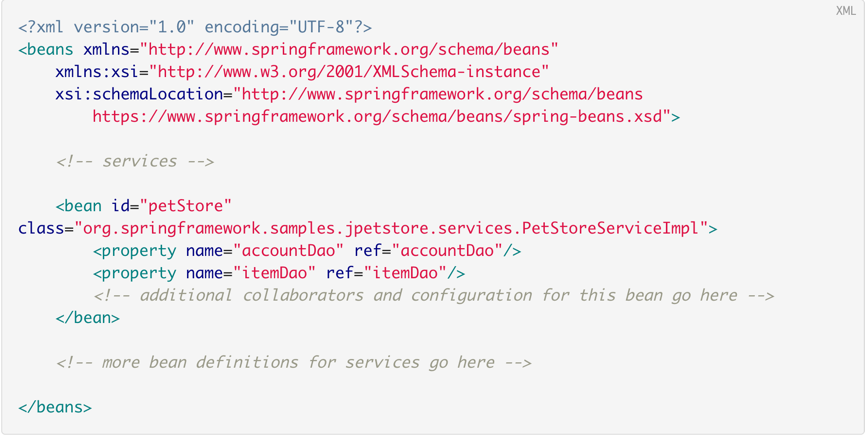
\includegraphics[width=1\textwidth]{code-3.png}
  \caption{Service object configuration}
  \label{fig:spring-code-3-en}
\end{figure}

In the preceding example, the service layer consists of the PetStoreServiceImpl class and two data access objects of the types JpaAccountDao and JpaItemDao (based on the JPA Object-Relational Mapping standard). The property nameelement refers to the name of the JavaBean property, and the ref element refers to the name of another bean definition. This linkage between id and ref elements expresses the dependency between collaborating objects. For details of configuring an object’s dependencies, see Dependencies.

It can be useful to have bean definitions span multiple XML files. Often, each individual XML configuration file represents a logical layer or module in your architecture.

You can use the application context constructor to load bean definitions from all these XML fragments. This constructor takes multiple Resource locations, as was shown in section. Alternatively, use one or more occurrences of the <import/> element to load bean definitions from another file or files. Picture \ref{fig:spring-code-4-en} shows how to do so:

\begin{figure}[!ht]
  \centering
  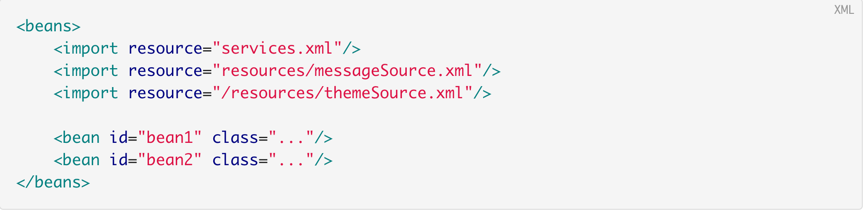
\includegraphics[width=1\textwidth]{code-4.png}
  \caption{Loading beans from other files}
  \label{fig:spring-code-4-en}
\end{figure}

In the preceding example, external bean definitions are loaded from three files: \hyphenation{services-\.-xml}, All location paths are relative to the definition file doing the importing, so \hyphenation{services-\.-xml} must be in the same directory or classpath location as the file doing the importing, while \hyphenation{message-Source-\.-xml} and \hyphenation{theme-Source-\.-xml} must be in a resources location below the location of the importing file. As you can see, a leading slash is ignored. However, given that these paths are relative, it is better form not to use the slash at all. The contents of the files being imported, including the top level <beans/> element, must be valid XML bean definitions, according to the Spring Schema.

It is possible, but not recommended, to reference files in parent directories using a relative "../" path. Doing so creates a dependency on a file that is outside the current application. In particular, this reference is not recommended for classpath: URLs, where the runtime resolution process chooses the “nearest” classpath root and then looks into its parent directory. Classpath configuration changes may lead to the choice of a different, incorrect directory.

You can always use fully qualified resource locations instead of relative paths: for example, file:C:/config/services.xml or classpath:/config/services.xml. However, be aware that you are coupling your application’s configuration to specific absolute locations. It is generally preferable to keep an indirection for such absolute locations — for example, through "\$\{…​\}" placeholders that are resolved against JVM system properties at runtime.

The namespace itself provices the import directive feature. Further configuration features beyond plain bean definitions are available in a selection of XML namespaces provided by Spring — for example, the context and util namespaces.

As a further example for externalized configuration metadata, bean definitions can also be expressed in Spring’s Groovy Bean Definition DSL, as known from the Grails framework. Typically, such configuration live in a ".groovy" file with the structure shown in the picture \ref{fig:spring-code-5-en}:

\begin{figure}[!ht]
  \centering
  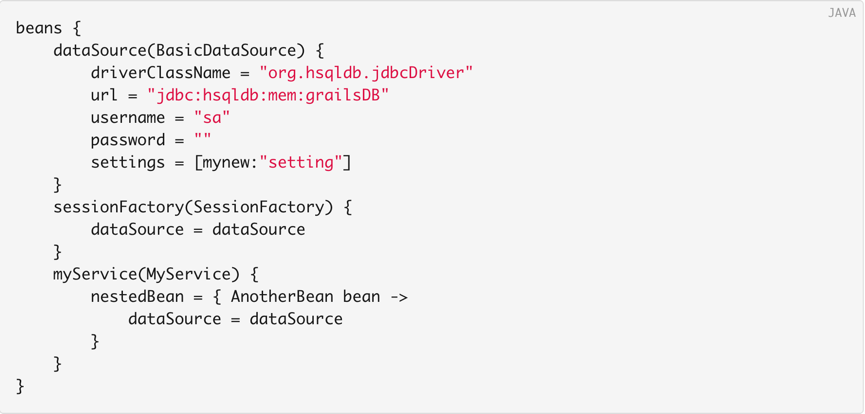
\includegraphics[width=1\textwidth]{code-5.png}
  \caption{Configure beans with Groovy}
  \label{fig:spring-code-5-en}
\end{figure}

This configuration style is largely equivalent to XML bean definitions and even supports Spring’s XML configuration namespaces. It also allows for importing XML bean definition files through an importBeans directive.

\xjtuappendixsubsection{Using the Container}
The ApplicationContext is the interface for an advanced factory capable of maintaining a registry of different beans and their dependencies. By using the method T getBean(String name, Class<T> requiredType), you can retrieve instances of your beans.

The ApplicationContext lets you read bean definitions and access them, as the picture \ref{fig:spring-code-6-en} shows:

\begin{figure}[!ht]
  \centering
  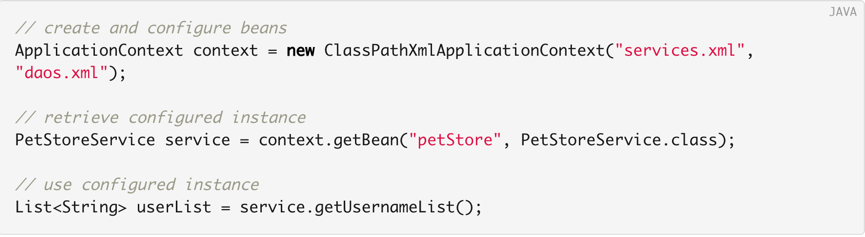
\includegraphics[width=1\textwidth]{code-6.png}
  \caption{Spring load configuration}
  \label{fig:spring-code-6-en}
\end{figure}

The ApplicationContext interface has a few other methods for retrieving beans, but, ideally, your application code should never use them. Indeed, your application code should have no calls to the getBean() method at all and thus have no dependency on Spring APIs at all. For example, Spring’s integration with web frameworks provides dependency injection for various web framework components such as controllers and JSF-managed beans, letting you declare a dependency on a specific bean through metadata (such as an autowiring annotation).

\xjtuappendixsection{Bean Overview}

A Spring IoC container manages one or more beans. These beans are created with the configuration metadata that you supply to the container (for example).

Within the container itself, these bean definitions are represented as BeanDefinition objects, which contain (among other information) the following metadata:

\begin{itemize}
  \item A package-qualified class name: typically, the actual implementation class of the bean being defined.
  \item Bean behavioral configuration elements, which state how the bean should behave in the container (scope, lifecycle callbacks, and so forth).
  \item References to other beans that are needed for the bean to do its work. These references are also called collaborators or dependencies.
  \item Other configuration settings to set in the newly created object — for example, the size limit of the pool or the number of connections to use in a bean that manages a connection pool.
\end{itemize}

This metadata translates to a set of properties that make up each bean definition. The table \ref{tab:bean-en}describes these properties:

\begin{table}[!ht]
  \centering
  \caption{Bean properties}
\label{tab:bean-en}
  \begin{tabularx}{\textwidth}{p{0.5\textwidth}<{\centering}p{0.5\textwidth}<{\centering}}
  \toprule
  Property & Explained in \\ \midrule
  Class & Instantiating Beans \\
  Name & Naming Beans \\ 
  Scope & Bean Scopes \\ 
  Constructor arguments & Dependency injection \\ 
  Properties & Dependency injection \\ 
  Autowiring mode & Autowiring Collaborators \\ 
  Lazy initialization mode & Lazy-initialized Beans \\ 
  initialization method & Initialization Callbacks \\
  Destruction method & Destruction Callbacks \\ \bottomrule
  \end{tabularx}
\end{table}

\xjtuappendixchapter{计算机源程序}

由于篇幅有限,仅列出系统核心源代码。

\xjtuappendixsection{后端源程序}

\xjtuappendixsubsection{用户注册与登录}

\begin{lstlisting}[ language=Java]
package com.suarezlin.controller;
import com.suarezlin.VO.UsersVO;
import com.suarezlin.pojo.Users;
import com.suarezlin.service.UserService;
import com.suarezlin.utils.CommonReturnType;
import io.swagger.annotations.Api;
import io.swagger.annotations.ApiImplicitParam;
import io.swagger.annotations.ApiOperation;
import org.apache.commons.lang3.StringUtils;
import org.springframework.beans.BeanUtils;
import org.springframework.beans.factory.annotation.Autowired;
import org.mindrot.jbcrypt.BCrypt;
import org.springframework.web.bind.annotation.PostMapping;
import org.springframework.web.bind.annotation.RequestBody;
import org.springframework.web.bind.annotation.RequestParam;
import org.springframework.web.bind.annotation.RestController;

import java.util.UUID;


@RestController
@Api(value = "用户注册/登录接口", tags = {"注册/登录 controller"})
public class RegisterLoginController extends BasicController {

    @Autowired
    UserService userService = null;

    @PostMapping("/register")
    @ApiOperation(value = "用户注册接口", notes = "用户注册接口")
    public CommonReturnType register(@RequestBody Users user) {

        // 判断用户名密码不为空
        if (StringUtils.isBlank(user.getUsername()) || StringUtils.isBlank(user.getPassword())) {
            return CommonReturnType.errorMsg("用户名或密码不能为空");
        }

        // 判断用户是否存在
        boolean isUserExist = userService.isUsernameExist(user.getUsername());
        if (isUserExist) {
            return CommonReturnType.errorMsg("用户名已存在");
        }

        // 保存用户
        user.setNickname(user.getUsername());
        try {
            user.setPassword(BCrypt.hashpw(user.getPassword(), BCrypt.gensalt()));
        } catch (Exception e) {
            return CommonReturnType.errorException(e.getMessage());
        }
        user.setFansCounts(0);
        user.setFollowCounts(0);
        user.setReceiveLikeCounts(0);

        userService.saveUser(user);
        user.setPassword("");

        UsersVO usersVO = setUserRedisSessionToken(user);
        return CommonReturnType.ok(usersVO);
    }

    public UsersVO setUserRedisSessionToken(Users user) {
        String uniqueToken = UUID.randomUUID().toString();
        redisOperator.set(USER_REDIS_SESSION + ":" + user.getId(), uniqueToken, 60 * 60 * 24 * 2);
        UsersVO usersVO = new UsersVO();
        BeanUtils.copyProperties(user, usersVO);
        usersVO.setUserToken(uniqueToken);
        return usersVO;
    }

    @PostMapping("/login")
    @ApiOperation(value = "用户登录接口", notes = "用户登录接口")
    public CommonReturnType login(@RequestBody Users user) {
//        try {
//            user.setPassword(MD5Utils.getMD5Str(user.getPassword()));
//        } catch (Exception e) {
//            return CommonReturnType.errorException(e.getMessage());
//        }
        user = userService.matchUser(user);
        if (user == null) {
            return CommonReturnType.errorMsg("用户名或密码错误");
        } else {
            user.setPassword("");
            UsersVO usersVO = setUserRedisSessionToken(user);
            return CommonReturnType.ok(usersVO);
        }
    }

    @PostMapping("/logout")
    @ApiOperation(value = "用户注销接口", notes = "用户注销接口")
    @ApiImplicitParam(name="userId", value = "用户 ID", required = true, dataType = "String", paramType = "query")
    public CommonReturnType logout(@RequestParam String userId) throws InterruptedException {
        redisOperator.del(USER_REDIS_SESSION + ":" + userId);
        return CommonReturnType.ok("注销成功");
    }
}

\end{lstlisting}

\xjtuappendixsubsection{视频服务接口}

\begin{lstlisting}[ language=Java]
  package com.suarezlin.controller;

  import com.suarezlin.VO.UsersVO;
  import com.suarezlin.pojo.Bgm;
  import com.suarezlin.pojo.Comments;
  import com.suarezlin.pojo.Users;
  import com.suarezlin.pojo.VO.VideosVO;
  import com.suarezlin.pojo.Videos;
  import com.suarezlin.service.BgmService;
  import com.suarezlin.service.VideoService;
  import com.suarezlin.utils.CommonReturnType;
  import com.suarezlin.utils.MergeVideoBgm;
  import com.suarezlin.utils.PagedResult;
  import com.suarezlin.utils.UUID;
  import io.swagger.annotations.*;
  import org.apache.commons.io.IOUtils;
  import org.apache.commons.lang3.StringUtils;
  import org.springframework.beans.BeanUtils;
  import org.springframework.beans.factory.annotation.Autowired;
  import org.springframework.beans.factory.annotation.Value;
  import org.springframework.data.domain.PageRequest;
  import org.springframework.web.bind.annotation.*;
  import org.springframework.web.multipart.MultipartFile;
  
  import java.io.*;
  import java.util.Date;
  import java.util.List;
  
  @RestController
  @RequestMapping("/video")
  @Api(value = "视频接口", tags = {"处理与视频相关操作的 controller"})
  public class VideoController {
  
      // 文件保存命名空间
      @Value("${com.suarezlin.filePath}")
      private String filePath;
  
      @Value("${com.suarezlin.ffmpegPath}")
      private String ffmpegPath;
  
      @Value("${com.suarezlin.ffprobePath}")
      private String ffprobePath;
  
      @Autowired
      private VideoService videoService;
  
      @Autowired
      private BgmService bgmService;
  
  
      @PostMapping(value = "/{userId}", headers = "content-type=multipart/form-data")
      @ApiOperation(value = "视频上传", notes = "用户上传视频的接口")
      @ApiImplicitParams({
              @ApiImplicitParam(name = "userId", value = "用户的 Id", required = true, dataType = "String", paramType = "path"),
              @ApiImplicitParam(name = "bgmId", value = "视频 bgm 的 Id", required = false, dataType = "String", paramType = "query"),
              @ApiImplicitParam(name = "videoSeconds", value = "上传视频的时长", required = true, dataType = "Double", paramType = "query"),
              @ApiImplicitParam(name = "videoWidth", value = "上传视频的宽度", required = true, dataType = "int", paramType = "query"),
              @ApiImplicitParam(name = "videoHeight", value = "上传视频的高度", required = true, dataType = "int", paramType = "query"),
              @ApiImplicitParam(name = "description", value = "上传视频的描述", required = false, dataType = "String", paramType = "query")
              //@ApiImplicitParam(name = "file", value = "上传视频文件", required = true, dataType = "MultipartFile", paramType = "body"),
      })
      public CommonReturnType upload(
                                     @PathVariable("userId") String userId,
                                     String bgmId,
                                     double videoSeconds,
                                     int videoWidth,
                                     int videoHeight,
                                     String description,
                                     @ApiParam(value = "上传视频", required = true) MultipartFile file
      ) throws IOException {
          if (StringUtils.isBlank(userId)) {
              return CommonReturnType.errorMsg("用户 Id 不能为空");
          }
  
          // 数据库中保存的视频路径
          String uploadPathDB = "/" + userId + "/video";
          FileOutputStream fileOutputStream = null;
          InputStream inputStream = null;
          try {
              if (file != null) {
                  String fileName = file.getOriginalFilename();
                  if (StringUtils.isBlank(fileName)) {
                      return CommonReturnType.errorMsg("视频名称不能为空");
                  } else {
                      // 文件上传绝对路径
                      String name = UUID.generateUUID();
                      String fileUploadPath = filePath + uploadPathDB + "/" + name + "." + fileName.split("\\.")[1];
                      // 设计数据库保存路径
                      uploadPathDB += ("/" + name + "." + fileName.split("\\.")[1]);
  
                      // 检测目录是否存在,若不存在则创建目录
                      File outFile = new File(fileUploadPath);
                      if (outFile.getParentFile() != null || !outFile.getParentFile().isDirectory()) {
                          // 创建目录
                          outFile.getParentFile().mkdirs();
                      }
  
                      // 文件输出
                      fileOutputStream = new FileOutputStream(fileUploadPath);
                      inputStream = file.getInputStream();
                      Videos video = new Videos();
                      video.setUserId(userId);
                      video.setVideoPath(uploadPathDB);
                      video.setVideoSeconds((float)videoSeconds);
                      video.setVideoHeight(videoHeight);
                      video.setVideoWidth(videoWidth);
                      video.setLikeCounts(0L);
                      video.setStatus(1);
                      video.setCreateTime(new Date());
                      if (bgmId != null && StringUtils.isNotBlank(bgmId)) {
                          video.setAudioId(bgmId);
                      }
                      if (description != null && StringUtils.isNotBlank(description)) {
                          video.setVideoDesc(description);
                      }
                      IOUtils.copy(inputStream, fileOutputStream);
  
                      // 获取视频截图作为封面
                      // 数据库保存路径
                      uploadPathDB = "/" + video.getUserId() + "/video/cover";
                      uploadPathDB += ("/" + name + ".jpg");
                      String coverFinalPath = filePath + uploadPathDB;
  
                      File cover = new File(coverFinalPath);
                      if (cover.getParentFile() == null || !cover.getParentFile().isDirectory()) {
                          cover.getParentFile().mkdirs();
                      }
  
                      MergeVideoBgm tool = new MergeVideoBgm(ffmpegPath);
                      tool.getScreenShot(fileUploadPath, coverFinalPath);
                      video.setCoverPath(uploadPathDB);
  
                      videoService.saveVideo(video);
  
  
                      // 若 bgmId 不为空,则需合并视频
                      if (StringUtils.isNotBlank(bgmId)) {
                          Bgm bgm = bgmService.getBgmById(bgmId);
                          String bgmPath = filePath + bgm.getPath();
                          String outputVideoName = video.getId() + ".mp4";
                          String outputVideoPath = filePath + "/" + userId + "/video" + "/" + outputVideoName;
                          System.out.println(bgmPath);
                          tool.convert(filePath + video.getVideoPath(), bgmPath, outputVideoPath, video.getVideoSeconds());
                          video.setVideoPath("/" + userId + "/video" + "/" + outputVideoName);
                          videoService.updateVideo(video);
                      }
  
                      return CommonReturnType.ok(video);
                  }
              } else {
                  return CommonReturnType.errorMsg("上传出错");
              }
          } catch (FileNotFoundException e) {
              e.printStackTrace();
              return CommonReturnType.errorMsg(e.getMessage());
          } catch (IOException e) {
              e.printStackTrace();
              return CommonReturnType.errorMsg(e.getMessage());
          } finally {
              try {
                  if (fileOutputStream != null) {
                      fileOutputStream.flush();
                      fileOutputStream.close();
                  }
              } catch (Exception e) {
                  return CommonReturnType.errorMsg(e.getMessage());
              }
          }
      }
  
      @PostMapping("/list")
      @ApiOperation(value = "分页查询视频", notes = "分页查询视频列表接口")
      @ApiImplicitParams({
              @ApiImplicitParam(name = "videos", value = "搜索体", required = false, dataType = "int", paramType = "query"),
              @ApiImplicitParam(name = "isSaveRecords", value = "为1搜索", required = false, dataType = "int", paramType = "query"),
              @ApiImplicitParam(name = "page", value = "当前页面数", required = false, dataType = "int", paramType = "query"),
              @ApiImplicitParam(name = "pageSize", value = "每页记录数", required = false, dataType = "int", paramType = "query")
      })
      public CommonReturnType getVideoList(@RequestBody Videos videos,@RequestParam(required = false) Integer isSaveRecords, Integer page, Integer pageSize) {
  
          if (page == null) {
              page = 1;
          }
          if (pageSize == null) {
              page = 10;
          }
  
          PagedResult pagedResult = videoService.getAllVideos(videos, isSaveRecords, page, pageSize);
  
          return CommonReturnType.ok(pagedResult);
      }
  
      @GetMapping("/hot")
      @ApiOperation(value = "查询热词", notes = "分页查询热词列表接口")
      public CommonReturnType getHot() {
  
  
          return CommonReturnType.ok(videoService.getHotWords());
      }
  
      @GetMapping("/{id}")
      @ApiOperation(value = "获取视频信息", notes = "通过视频 id 获取视频信息")
      @ApiImplicitParam(name = "id", value = "所查询视频的 id", required = true, dataType = "String", paramType = "path")
      public CommonReturnType getVideo(@PathVariable("id") String id) {
          if (StringUtils.isBlank(id)) {
              return CommonReturnType.errorMsg("视频 id 不能为空");
          }
          Videos video = videoService.getVideoById(id);
          return CommonReturnType.ok(video);
      }
  
      @PostMapping(value = "/like")
      public CommonReturnType userLike(String userId, String videoId, String videoCreaterId) {
          videoService.userLikeVideo(userId, videoId, videoCreaterId);
          return CommonReturnType.ok();
      }
  
      @PostMapping(value = "/notlike")
      public CommonReturnType userNotLike(String userId, String videoId, String videoCreaterId) {
          videoService.userNotLikeVideo(userId, videoId, videoCreaterId);
          return CommonReturnType.ok();
      }
  
  //    @GetMapping("/getComment")
  //    public CommonReturnType getComment() {
  //
  //    }
  
      @GetMapping("/getVideo")
      public CommonReturnType getUserVideos(String publisherId, Integer page, Integer pageSize) {
          if (StringUtils.isBlank(publisherId) || StringUtils.isEmpty(publisherId)) {
              return CommonReturnType.errorMsg("用户 Id 不能为空");
          }
          PagedResult pagedResult = videoService.getUserVideos(publisherId, page, pageSize);
          return CommonReturnType.ok(pagedResult);
      }
  
      @GetMapping("/getLikeVideo")
      public CommonReturnType getLikeVideo(String userId, Integer page, Integer pageSize) {
          if (StringUtils.isBlank(userId) || StringUtils.isEmpty(userId)) {
              return CommonReturnType.errorMsg("用户 Id 不能为空");
          }
          PagedResult pagedResult = videoService.getUserLikeVideos(userId, page, pageSize);
          return CommonReturnType.ok(pagedResult);
      }
  
      @GetMapping("/getFollowVideo")
      public CommonReturnType getFollowVideo(String userId, Integer page, Integer pageSize) {
          if (StringUtils.isBlank(userId) || StringUtils.isEmpty(userId)) {
              return CommonReturnType.errorMsg("用户 Id 不能为空");
          }
          PagedResult pagedResult = videoService.getUserFollowVideos(userId, page, pageSize);
          return CommonReturnType.ok(pagedResult);
      }
  
      @PostMapping("/delete")
      public CommonReturnType deleteVideo(String videoId) {
          if (StringUtils.isBlank(videoId) || StringUtils.isEmpty(videoId)) {
              return CommonReturnType.errorMsg("视频 Id 不能为空");
          }
          Videos video = videoService.getVideoById(videoId);
          videoService.deleteVideo(videoId);
          File videoFile = new File(filePath + video.getVideoPath());
          File coverFile = new File(filePath + video.getCoverPath());
          if (!videoFile.delete()) {
              return CommonReturnType.errorMsg("删除失败");
          }
          if (!coverFile.delete()) {
              return CommonReturnType.errorMsg("删除失败");
          }
          return CommonReturnType.ok();
      }
  
      @PostMapping("/comments/add")
      public CommonReturnType addComments(@RequestBody Comments comment) {
          videoService.addComment(comment);
          return CommonReturnType.ok();
      }
  
      @GetMapping("/comments/get")
      public CommonReturnType getComments(String videoId, Integer page, Integer pageSize) {
          if (StringUtils.isBlank(videoId) || StringUtils.isEmpty(videoId)) {
              return CommonReturnType.errorMsg("视频 Id 不能为空");
          }
          PagedResult pagedResult = videoService.getVideoComments(videoId, page, pageSize);
          return CommonReturnType.ok(pagedResult);
      }
  
  }
  
\end{lstlisting}

\xjtuappendixsubsection{视频处理}

\begin{lstlisting}[ language=Java]
  package com.suarezlin.utils;

  import java.io.BufferedReader;
  import java.io.IOException;
  import java.io.InputStream;
  import java.io.InputStreamReader;
  import java.util.ArrayList;
  import java.util.List;
  
  public class MergeVideoBgm {
  
      private String ffmpegPath;
  
      public MergeVideoBgm() {
  
      }
  
      public MergeVideoBgm(String ffmpegPath) {
          this.ffmpegPath = ffmpegPath;
      }
  
      public String getFfmpegPath() {
          return ffmpegPath;
      }
  
      public void setFfmpegPath(String ffmpegPath) {
          this.ffmpegPath = ffmpegPath;
      }
  
      public void convert(String inputVideoPath, String inputBgmPath, String outputVideoPath, float seconds) throws IOException {
          List<String> commands = new ArrayList<>();
          commands.add(ffmpegPath);
          commands.add("-i");
          commands.add(inputVideoPath);
          commands.add("-i");
          commands.add(inputBgmPath);
          commands.add("-t");
          commands.add(String.valueOf(seconds));
          commands.add("-y");
          commands.add(outputVideoPath);
  
  //        for (String s : commands) {
  //            System.out.print(s);
  //        }
  
          ProcessBuilder builder = new ProcessBuilder(commands);
          Process process = builder.start();
          InputStream errorStream = process.getErrorStream();
          InputStreamReader inputStreamReader = new InputStreamReader(errorStream);
          BufferedReader bufferedReader = new BufferedReader(inputStreamReader);
          String line = "";
  
          while ((line = bufferedReader.readLine()) != null) {
              //System.out.println(line);
          }
  
          if (bufferedReader != null) {
              bufferedReader.close();
          }
          if (inputStreamReader != null) {
              inputStreamReader.close();
          }
          if (errorStream != null) {
              errorStream.close();
          }
      }
  
      public void getScreenShot(String inputVideoPath, String outputImgPath) throws IOException {
          // ffmpeg -i demo.mp4 -ss 00:00:01 -vframes 1 -y out.jpg
          List<String> commands = new ArrayList<>();
          commands.add(ffmpegPath);
          commands.add("-i");
          commands.add(inputVideoPath);
          commands.add("-ss");
          commands.add("00:00:01");
          commands.add("-vframes");
          commands.add("1");
          commands.add("-y");
          commands.add("-q:v");
          commands.add("2");
          commands.add(outputImgPath);
  
  //        for (String s : commands) {
  //            System.out.print(s);
  //        }
  
          ProcessBuilder builder = new ProcessBuilder(commands);
          Process process = builder.start();
          InputStream errorStream = process.getErrorStream();
          InputStreamReader inputStreamReader = new InputStreamReader(errorStream);
          BufferedReader bufferedReader = new BufferedReader(inputStreamReader);
          String line = "";
  
          while ((line = bufferedReader.readLine()) != null) {
              //System.out.println(line);
          }
  
          if (bufferedReader != null) {
              bufferedReader.close();
          }
          if (inputStreamReader != null) {
              inputStreamReader.close();
          }
          if (errorStream != null) {
              errorStream.close();
          }
      }
  
      public static void main(String[] args) throws IOException {
          MergeVideoBgm ffMpeg = new MergeVideoBgm("/Users/hayashikoushi/Downloads/ffmpeg-static/bin/ffmpeg");
          ffMpeg.convert("/Users/hayashikoushi/Downloads/IMG_0908.MOV", "/Users/hayashikoushi/Documents/code/GraduationProject/ProjectFile/bgm/Panzerlied(少战).mp3","/Users/hayashikoushi/Downloads/新视频.avi", 3);
  
      }
  
  }
  
\end{lstlisting}